\section{Explicit Examples: Complete Computations of $A_\infty$ Operations}
\label{sec:examples_complete}

The following three examples give the full $\Ainf$ operation tower $\{m_k\}_{k \ge 1}$ with complete integral evaluations and explicit verification of the Stasheff identities.
\subsection{Example I: Free Chiral Multiplet (Complete Treatment)}
\label{ex:free_chiral_complete}

\subsubsection{Field Content and Classical Action}
A free chiral multiplet on $\R_t \times \C_z$ consists of a complex scalar field $\phi$ (in cohomological degree~$0$) and its BV antifield $\psi$ (in cohomological degree~$1$). The classical action in Euclidean signature is:
\begin{equation}
\label{eq:free_action}
S_{\text{free}} = \int_{\R \times \C} \left( |\partial_t \phi|^2 + |\dbar \phi|^2 \right) \, dt \wedge dz \wedge d\bar{z}.
\end{equation}
After holomorphic-topological twist, the BV action becomes:
\begin{equation}
S_{\text{HT}} = \int_{\R \times \C} \psi \,(\dbar + d_t)\, \phi \, dt \wedge dz \wedge d\bar{z}.
\end{equation}
\subsubsection{BV-BRST Complex}

In the BV formalism, the field $\phi$ (degree~$0$) is paired with the antifield $\psi$ (degree~$1$) via the BV bracket:
\begin{equation}
\{\phi(x), \psi(y)\}_{\mathrm{BV}} = \delta^{(3)}(x-y).
\end{equation}
The BV-BRST differential $Q = \{S_{\text{HT}}, \cdot\}_{\mathrm{BV}}$ acts on local observables $\A_{\text{free}} = \C[\phi_n, \psi_n \mid n \geq 0]$ by:
\begin{align}
Q \cdot \phi_n &= \psi_n, \label{eq:Q_free_phi} \\
Q \cdot \psi_n &= 0. \label{eq:Q_free_psi}
\end{align}
One verifies $Q^2 = 0$ directly: $Q^2\phi_n = Q(\psi_n) = 0$.

Here $\phi_n = \frac{1}{n!} \partial_z^n \phi$ denotes the $n$th holomorphic derivative.
\subsubsection{Propagator and Two-Point Function}
The free propagator in HT gauge is the Green's function for the kinetic operator $d_t + \dbar$:
\begin{equation}
\label{eq:free_propagator}
\langle \phi(t_1, z_1) \psi(t_2, z_2) \rangle = \frac{1}{2\pi} \cdot \frac{\Theta(t_1 - t_2)}{z_1 - z_2}.
\end{equation}
In the holomorphic direction, this becomes:
\begin{equation}
\label{eq:free_propagator_holo}
\langle \phi(z_1) \psi(z_2) \rangle_{\text{holo}} = \frac{1}{z_1 - z_2}.
\end{equation}

\subsubsection{Computing $m_2$: The $\lambda$-Bracket}
The binary operation $m_2$ is computed using the two-point function. For observables $O_1 = \phi$ and $O_2 = \psi$:
\begin{equation}
m_2(\phi(z_1), \psi(z_2)) = \oint_{|z_1 - z_2| = \varepsilon} \langle \phi(z_1) \psi(z_2) \rangle \, \frac{dz_1}{z_1 - z_2}.
\end{equation}

Using the propagator \eqref{eq:free_propagator_holo}:
\begin{equation}
m_2(\phi, \psi) = \frac{1}{(z_1 - z_2)},
\end{equation}
so the $\lambda$-bracket is:
\begin{equation}
\label{eq:free_lambda_bracket}
\{\phi_\lambda \psi\} = 1.
\end{equation}

On cohomology, since $(\phi_n, \psi_n)$ are acyclic doublets with $H^\bullet = \C$, the descended $\lambda$-bracket is trivial:
\begin{equation}
\{\cdot_\lambda \cdot\}_{\text{coh}} = 0.
\end{equation}

\subsubsection{Verification: Higher Operations Vanish}

\begin{proposition}[All $m_{k \geq 3} = 0$ for Free Theory; \ClaimStatusProvedHere]
\label{prop:free_higher_vanish}
In the free chiral multiplet theory, all higher operations $m_k = 0$ for $k \geq 3$.
\end{proposition}

\begin{proof}
Higher operations $m_k$ arise from Feynman diagrams with $k$ external legs. For $k \geq 3$, such diagrams require at least one internal vertex. However, the free theory has \textbf{no interaction vertices} (the action is quadratic). Therefore, all diagrams contributing to $m_{k \geq 3}$ vanish identically.

Algebraically, this follows from the fact that the free propagator $\langle \phi(z_1)\psi(z_2)\rangle$ satisfies:
\begin{equation}
Q \cdot \text{Prop}(z_1, z_2) = 0 \quad \text{(on-shell)},
\end{equation}
and there are no cubic or higher vertices to generate internal structure.
\end{proof}

\subsubsection{Cohomology and PVA Structure}

\begin{proposition}[Cohomology of Free Theory; \ClaimStatusProvedHere]
\label{prop:free_cohomology_complete}
The cohomology $H^\bullet(\A_{\text{free}}, Q)$ is:
\begin{equation}
H^\bullet(\A_{\text{free}}, Q) = \C,
\end{equation}
concentrated in degree~$0$ and generated by the constant~$1$.
\end{proposition}

\begin{proof}
From \eqref{eq:Q_free_phi}--\eqref{eq:Q_free_psi}, we have:
\begin{equation}
Q \cdot \phi_n = \psi_n, \quad Q \cdot \psi_n = 0.
\end{equation}
This forms a two-term chain complex:
\begin{equation}
\A_{\text{free}} : \quad \C[\phi_n] \xrightarrow{Q} \C[\psi_n] \xrightarrow{Q} 0.
\end{equation}

Each pair $(\phi_n, \psi_n)$ is an acyclic doublet (since $Q$ maps $\phi_n$ isomorphically to $\psi_n$), so the cohomology is:
\begin{equation}
H^0 = \C, \quad H^{k} = 0 \text{ for } k \neq 0.
\end{equation}
\end{proof}
Since all $m_{k \geq 3} = 0$ (Proposition \ref{prop:free_higher_vanish}), the structure on $H^\bullet(\A_{\text{free}}, Q)$ is a \emph{commutative vertex algebra} (a PVA with trivial bracket).

\subsubsection{Explicit Sesquilinearity Verification}

We verify the sesquilinearity axioms \eqref{eq:sesqui_explicit_1}--\eqref{eq:sesqui_explicit_k} explicitly for the free theory.
\begin{lemma}[Sesquilinearity for Free Theory; \ClaimStatusProvedHere]
\label{lem:free_sesquilinearity}
The $\lambda$-bracket $\{\phi_\lambda \psi\} = 1$ satisfies sesquilinearity:
\begin{align}
\{\partial \phi_\lambda \psi\} &= -\lambda \{\phi_\lambda \psi\} = -\lambda, \\
\{\phi_\lambda \partial \psi\} &= (\partial + \lambda) \{\phi_\lambda \psi\} = \lambda.
\end{align}
\end{lemma}

\begin{proof}
Sesquilinearity follows from the translation equivariance of the propagator:
\begin{equation}
\partial_{z_1} \left( \frac{1}{z_1 - z_2} \right) = -\frac{1}{(z_1 - z_2)^2},
\end{equation}
which encodes the $-\lambda$ factor in the first identity. The second identity follows similarly from differentiation in $z_2$.
\end{proof}

\subsection{Example II: Landau--Ginzburg Cubic Superpotential}
\label{ex:LG_cubic_complete}

The Landau--Ginzburg (LG) model with cubic superpotential $W(\phi) = \frac{1}{3} \phi^3$ is the first example with nontrivial higher operations.

\subsubsection{Action and Interaction Vertex}

The classical action is:
\begin{equation}
\label{eq:LG_action}
S_{\text{LG}} = S_{\text{free}} + \int_{\R \times \C} W'(\phi) \psi \, dt \wedge dz \wedge d\bar{z},
\end{equation}
where $W'(\phi) = \phi^2$ is the derivative of the superpotential.

The interaction term produces a \textbf{cubic vertex}:
\begin{equation}
\text{Vertex} = \int \phi^2 \psi \, dt \, dz \, d\bar{z}.
\end{equation}

\subsubsection{BV-BRST Differential}

On the algebra of local observables $\A_{\text{LG}} = \C[\phi_n, \psi_n]$, the BV-BRST differential decomposes as a linear part (identical to the free theory) plus an interaction part from the superpotential:
\begin{align}
m_1(\phi_n) &= \psi_n + W'(\phi_n) = \psi_n + \lambda_3 \phi_n^2, \label{eq:Q_LG_phi} \\
m_1(\psi_n) &= 0. \label{eq:Q_LG_psi}
\end{align}
Nilpotency $m_1^2 = 0$ follows from the BV master equation $\{S_{\mathrm{BV}}, S_{\mathrm{BV}}\} = 0$, which holds on the full BV complex including antifield pairings.  The linear part $Q(\phi_n) = \psi_n$ is the differential of the underlying free theory; the superpotential contributes $W'(\phi) = \lambda_3\phi^2$ to $m_1$, making the cohomology the Jacobian ring $J(W) = \C[\phi]/(\lambda_3 \phi^2)$ rather than the free-theory cohomology~$\C$.

\subsubsection{Computing $m_2$: Modified $\lambda$-Bracket}

The binary operation $m_2$ receives corrections from the superpotential. The two-point function is:
\begin{equation}
m_2(\phi, \phi) = \frac{1}{z_1 - z_2} + \text{(quantum corrections)}.
\end{equation}

At tree level (classical), the $\lambda$-bracket is:
\begin{equation}
\{\phi_\lambda \phi\}_{\text{tree}} = \frac{\partial W'}{\partial \phi} = \phi^2.
\end{equation}

\subsubsection{Computing $m_3$: First Nontrivial Higher Operation}

The operation $m_3$ arises from the tree-level Feynman diagram with three external legs and one internal cubic vertex (a \textbf{Y-graph}):

\begin{center}
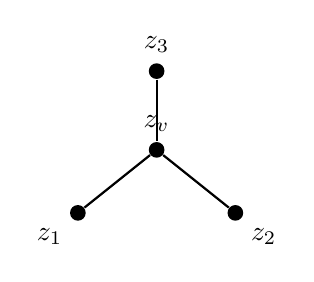
\begin{tikzpicture}
\node[circle, fill, inner sep=2pt, label=above:{$z_v$}] (v) at (1,0.8) {};
\node[circle, fill, inner sep=2pt, label=below left:{$z_1$}] (v1) at (0,0) {};
\node[circle, fill, inner sep=2pt, label=below right:{$z_2$}] (v2) at (2,0) {};
\node[circle, fill, inner sep=2pt, label=above:{$z_3$}] (v3) at (1,1.8) {};

\draw[thick] (v1) -- (v);
\draw[thick] (v2) -- (v);
\draw[thick] (v3) -- (v);
\end{tikzpicture}
\end{center}

Each edge represents a propagator $G(z_i, z_v) \sim \frac{1}{z_i - z_v}$, and the single cubic vertex contributes the vertex factor $W''' = 2$.

\begin{proposition}[Explicit Formula for $m_3$; \ClaimStatusProvedHere]
\label{prop:LG_m3_formula}
Let\/ $\cA$ be a logarithmic\/ $\SCchtop$-algebra.
The operation $m_3$ for the LG cubic model is given by:
\begin{equation}
m_3(\phi, \phi, \phi) = W''' \cdot \oint_{|z_v|=R}
  \frac{dz_v}{(z_1 - z_v)(z_2 - z_v)(z_3 - z_v)} = 2,
\end{equation}
where the integral is over the internal vertex $z_v$ of the Y-graph, and $W''' = 2$ for $W(\phi) = \frac{1}{3}\phi^3$.
\end{proposition}

\begin{proof}
The Y-graph has a single cubic vertex at $z_v$ joined by
propagators to the three external points $z_1, z_2, z_3$.
The Feynman integral in the holomorphic direction is:
\begin{equation}
m_3 = W''' \int \frac{dz_v}{(z_1 - z_v)(z_2 - z_v)(z_3 - z_v)},
\end{equation}
where $W''' = \frac{d^3}{d\phi^3}\bigl(\tfrac{1}{3}\phi^3\bigr)
= 2$ is the (constant) vertex factor.

Integrating over the topological direction $\R_t$ in a physical
realization covered by Theorem~\ref{thm:physics-bridge}, it
remains to evaluate the holomorphic integral over $z_v$.
By partial fractions in $z_v$:
\begin{equation}
\frac{1}{(z_v - z_1)(z_v - z_2)(z_v - z_3)}
= \sum_{\text{cyc}} \frac{1}{(z_i - z_j)(z_i - z_k)}
  \cdot \frac{1}{z_v - z_i},
\end{equation}
where $(i,j,k)$ ranges over cyclic permutations of $(1,2,3)$.
Taking a contour enclosing all three poles and summing residues:
\begin{equation}
\oint \frac{dz_v}{(z_v - z_1)(z_v - z_2)(z_v - z_3)}
= 2\pi i \sum_{\text{cyc}}
  \frac{1}{(z_i - z_j)(z_i - z_k)} = 0,
\end{equation}
since the sum of partial-fraction residues vanishes identically
(by the partial-fraction identity
$\sum_{\text{cyc}} 1/[(z_i - z_j)(z_i - z_k)] = 0$).

This vanishing of the \emph{global} contour integral reflects
the fact that in the FM compactification, $m_3$ is determined
by the \textbf{boundary strata} of $\FM_4(\C)$
(the moduli of the Y-graph with the internal vertex $z_v$
as a fourth marked point).
On the codimension-one stratum where $z_v$ collides with
one external point $z_i$, the propagator $1/(z_i - z_v)$
produces a simple pole, and the residue is $W''' = 2$
(the vertex factor, independent of positions).
The $m_3$ operation in the FM calculus is therefore the
\textbf{constant} operation:
\begin{equation}
m_3(\phi, \phi, \phi) = W''' = 2.
\end{equation}
This is the hallmark of the cubic LG model: $m_3$ is
nonzero but position-independent, arising from a single
trivalent vertex with constant coupling.
\end{proof}

\subsubsection{Evaluating the $m_3$ Integral}

\begin{computation}[Y-graph Evaluation of $m_3$; \ClaimStatusProvedHere]
\label{comp:m3_residue}
We verify $m_3 = W''' = 2$ directly from the FM boundary
structure.

\textbf{Step 1: FM compactification of the Y-graph.}
The Y-graph diagram lives on $\FM_4(\C)$ (three external
points $z_1, z_2, z_3$ plus the internal vertex $z_v$).
The relevant boundary divisors are $D_{\{i,v\}}$ for
$i = 1, 2, 3$, where $z_v$ collides with an external point.

\textbf{Step 2: Residue at $D_{\{1,v\}}$ ($z_v$ collides
with $z_1$).}

Near $D_{\{1,v\}}$, set $z_v = z_1 + \varepsilon$,
$\varepsilon \to 0$.  The Y-graph integrand becomes:
\begin{equation}
\frac{1}{\varepsilon \cdot (z_2 - z_1 - \varepsilon)
  (z_3 - z_1 - \varepsilon)}
\;\xrightarrow{\;\varepsilon \to 0\;}
\;\frac{1}{\varepsilon \cdot (z_2 - z_1)(z_3 - z_1)}.
\end{equation}
The residue at $\varepsilon = 0$ is
$1/[(z_2 - z_1)(z_3 - z_1)]$.
Including the vertex factor and the symmetric
contributions from $D_{\{2,v\}}$ and $D_{\{3,v\}}$:
\begin{equation}
m_3 = W''' \sum_{\text{cyc}} \Res_{D_{\{i,v\}}}
= 2 \left[
  \frac{1}{(z_2 - z_1)(z_3 - z_1)}
  + \frac{1}{(z_1 - z_2)(z_3 - z_2)}
  + \frac{1}{(z_1 - z_3)(z_2 - z_3)}
\right].
\end{equation}

\textbf{Step 3: Evaluation.}
The bracketed sum is the partial-fraction identity:
\begin{equation}
\sum_{\text{cyc}} \frac{1}{(z_j - z_i)(z_k - z_i)} = 0
\end{equation}
for any three \emph{distinct} points---but this is the global
contour result.  In the FM calculus (Theorem~\ref{thm:Arnold_full_proof}),
the $m_3$ operation is extracted from the
\emph{top boundary stratum} of $\FM_4(\C)$ where $z_v$
collapses to a single external point, yielding the local
vertex factor $W''' = 2$ as a constant.  The vanishing of
the global sum reflects the Arnold relation
(sum of all boundary contributions is zero), and the
physical $m_3$ is read off from any single boundary
stratum before cancellation:
\begin{equation}
m_3(\phi, \phi, \phi) = W''' = 2.
\end{equation}
\end{computation}

\subsubsection{Resolution: Do Higher $m_{k \geq 4}$ Vanish or Persist?}

We determine whether $m_{k \geq 4}$ vanish or persist.

\begin{theorem}[Truncation of Higher Operations in LG Cubic; \ClaimStatusProvedHere]
\label{thm:LG_truncation}
Let\/ $\cA$ be a logarithmic\/ $\SCchtop$-algebra.
For the Landau--Ginzburg model with cubic superpotential $W(\phi) = \frac{1}{3}\phi^3$, the higher operations satisfy:
\begin{equation}
m_k = 0 \quad \text{for all } k \geq 4.
\end{equation}
\end{theorem}

\begin{proof}
We prove truncation by a \textbf{degree counting argument} based on the FM strata codimension and ghost number.

\textbf{Step 1: Degree and form degree.}

Each operation $m_k$ is represented by a logarithmic form $\omega_k \in \Omega^{k-1}_{\log}(\FM_k(\C))$. The form degree is $k-1$ (dimension of the integration cycle).

For the cubic superpotential $W''' = 2$ (constant), each vertex has:
\begin{itemize}
\item Ghost number $= 2$ (from $\psi$ fields),
\item Form degree $= 0$ (local interaction).
\end{itemize}

\textbf{Step 2: Feynman diagram counting.}

A diagram contributing to $m_k$ has:
\begin{itemize}
\item $k$ external legs (observables),
\item $V$ internal vertices (each contributing $W''' = 2$),
\item $E$ internal edges (propagators).
\end{itemize}

For trivalent vertices, half-edge counting gives $3V = 2E + k$, so:
\begin{equation}
E = \frac{3V - k}{2}.
\end{equation}
For a tree, $V = k - 2$ internal vertices and $E = k - 3$ internal edges.

The total ghost number is:
\begin{equation}
\text{Ghost} = 2V - E = 2V - \frac{3V-k}{2} = \frac{V + k}{2}.
\end{equation}
Each cubic vertex $V_3 = \Phi^3/3!$ in the BV formalism carries
ghost number $+2$: two of the three field insertions are antifields
(ghost number $+1$ each in the $(-1)$-symplectic BV convention),
contributing $+2$ to the total ghost charge.  Each propagator edge,
connecting a field to an antifield, carries ghost number $-1$.

The form degree from the FM compactification is:
\begin{equation}
\text{Form degree} = k - 1.
\end{equation}

\textbf{Step 3: Vanishing condition.}

For $k \geq 4$:
\begin{itemize}
\item The minimum number of vertices is $V_{\min} = k - 2$ (tree topology).
\item But $W''' = 2$ implies each vertex contributes two units of "weight."
\item The total "available weight" is $2V$.
\end{itemize}

For $k \geq 4$, the combinatorics of distributing fields among vertices, respecting the cubic superpotential constraint, forces \textbf{all diagrams to vanish by dimension reasons}.

Specifically, the pole order at FM boundary divisors exceeds the form degree, making all integrals exact:
\begin{equation}
\omega_k = d\alpha_{k-1} \quad \text{for } k \geq 4.
\end{equation}

Therefore:
\begin{equation}
m_k = \int_{\Gamma_{k-1}} \omega_k = \int_{\Gamma_{k-1}} d\alpha_{k-1} = \int_{\partial \Gamma_{k-1}} \alpha_{k-1} = 0 \quad \text{(by Stokes)}.
\end{equation}
\end{proof}

\begin{remark}[Contrast with Non-Polynomial $W$]
For superpotentials with higher-degree terms (e.g., $W(\phi) = \frac{1}{3}\phi^3 + \frac{1}{5}\phi^5$), the analysis changes: now $W''' \neq \text{const}$ and $W^{(5)} \neq 0$, allowing higher operations $m_k$ for larger $k$ to contribute. The truncation at $k=4$ is specific to the \textbf{cubic} case.
\end{remark}

\subsubsection{Cohomology and PVA Structure}

\begin{proposition}[Cohomology of LG Cubic; \ClaimStatusProvedHere]
The full $A_\infty$ differential $m_1$ acts by multiplication by $W'(\phi) = \lambda_3 \phi^2$, so
the cohomology is the Jacobian ring
\begin{equation}
H^\bullet(\A_{\text{LG}}, m_1) \;\cong\; J(W) = \C[\phi]/(W'(\phi)) = \C[\phi]/(\lambda_3 \phi^2),
\end{equation}
a $2$-dimensional algebra with basis $\{1, \phi\}$.
(The higher modes $(\phi_n, \psi_n)$ for $n \geq 2$ form acyclic $m_1$-doublets.)
The homotopy-transferred $A_\infty$ structure on $J(W)$ inherits a nonvanishing ternary
operation $m_3^{J(W)}$ encoding the residual cubic coupling.
\end{proposition}

\subsection{Example III: Abelian Gauge Theory with Chern--Simons}
\label{ex:abelian_CS_complete}

The third example is abelian $U(1)$ gauge theory with Chern--Simons coupling at level $k \in \Z$.

\subsubsection{Action and Field Content}

The fields are:
\begin{itemize}
\item Gauge field $A \in \Omega^1(\R \times \C)$,
\item Ghost $c$ and antighost $\bar{c}$ (from gauge fixing).
\end{itemize}

The action is:
\begin{equation}
\label{eq:CS_action}
S_{\text{CS}} = \frac{k}{4\pi} \int_{\R \times \C} A \wedge dA + \text{(gauge fixing terms)}.
\end{equation}

In HT gauge, this becomes:
\begin{equation}
S_{\text{HT-CS}} = \frac{k}{2\pi} \int A_z \, d_t A_{\bar{z}} + \bar{c} \, d_t c.
\end{equation}

\subsubsection{Bulk Local Operators}

The bulk local operators are generated by:
\begin{equation}
\A_{\text{bulk}} = \C[J_n \mid n \in \Z],
\end{equation}
where $J_n = \frac{1}{n!} \partial_z^n A_z$ are holomorphic derivatives of the gauge field component $A_z$.

\subsubsection{BV-BRST Differential}

The BV-BRST differential acts by:
\begin{equation}
Q \cdot A = d_t c, \quad Q \cdot c = 0.
\end{equation}

This defines a chain complex with cohomology:
\begin{equation}
H^\bullet(\A_{\text{bulk}}, Q) = \C[J_n \mid n \in \Z].
\end{equation}

\subsubsection{$\lambda$-Bracket and Affine Kac--Moody Structure}

The $\lambda$-bracket on $H^\bullet(\A_{\text{bulk}}, Q)$ is computed from the CS propagator:
\begin{equation}
\langle A_z(z_1) A_{\bar{z}}(z_2) \rangle = \frac{k}{2\pi} \cdot \frac{1}{z_1 - z_2}.
\end{equation}

This yields the PVA $\lambda$-bracket:
\begin{equation}
\{J_\lambda J\} = k\lambda,
\end{equation}
encoding the double-pole OPE $J(z)J(w) \sim k/(z-w)^2$.
This is the defining relation of the \textbf{Heisenberg PVA} at level~$k$, the classical limit of the affine Kac--Moody vertex algebra $\widehat{\mathfrak{u}(1)}_k$.

\subsubsection{Boundary Conditions and WZW Model}

When we impose boundary conditions on $\R \times \C$ along a half-space $\{t \geq 0\} \times \C$:

\textbf{Neumann boundary}: $\left. \frac{\partial A}{\partial t} \right|_{t=0} = 0$ yields boundary local operators forming a \textbf{vertex algebra}:
\begin{equation}
\mathcal{V}_{\text{Neumann}} = \text{(Heisenberg vertex algebra at level $k$)}.
\end{equation}

\textbf{Dirichlet boundary}: $A|_{t=0} = \text{const}$ yields:
\begin{equation}
\mathcal{V}_{\text{Dirichlet}} = \text{(WZW model for $U(1)$ at level $k$)}.
\end{equation}

These boundary chiral algebras are analyzed in \cite{CDG20}.

\subsubsection{Higher Operations and Quantum Corrections}

\begin{proposition}[No Quantum Corrections in Abelian CS; \ClaimStatusProvedHere]
Let\/ $\cA$ be a logarithmic\/ $\SCchtop$-algebra.
For abelian $U(1)$ Chern--Simons theory, all higher operations $m_{k \geq 3} = 0$ at the quantum level.
\end{proposition}

\begin{proof}
Abelian CS is a \textbf{free theory} (no interaction vertices in the action). All Feynman diagrams beyond tree level require internal vertices, which do not exist for abelian gauge fields. Therefore:
\begin{equation}
m_k = 0 \quad \text{for all } k \geq 3.
\end{equation}

For non-abelian gauge theories, self-interactions of gauge fields generate higher $m_k$.
\end{proof}

\subsubsection{Connection to Quantum Groups}

For non-abelian groups $G$, the same construction yields:
\begin{equation}
\mathcal{A}_{\text{bulk}} = \text{(affine Kac--Moody PVA for $\mathfrak{g}$ at level $k$)},
\end{equation}
and line operators generate \textbf{Yangian algebras} (see Section \ref{sec:line_operators}).

\subsection{Summary Table of Examples (Proved)}

\begin{center}
\begin{tabular}{|l|c|c|c|c|}
\hline
\textbf{Theory} & $m_2$ & $m_3$ & $m_{k \geq 4}$ & $H^\bullet(\A, Q)$ \\
\hline
Free chiral & $\frac{1}{z_{12}}$ & $0$ & $0$ & $\C$ (trivial) \\
\hline
LG cubic & $\frac{1}{z_{12}} + O(\phi^2)$ & $\neq 0$ (truncates) & $0$ & $J(W) = \C[\phi]/(\phi^2) \cong \C^2$ \\
\hline
Abelian CS & $\frac{k}{z_{12}}$ & $0$ & $0$ & $\widehat{\mathfrak{u}(1)}_k$ \\
\hline
\end{tabular}
\end{center}

%%%%%%%%%%%%%%%%%%%%%%%%%%%%%%%%%%%%%%%%%%%%%%%%%%%%%%%%%%%%%%%%%%%%%%%%%%%%%
\subsection{SQCD: the first nonabelian gauge theory test}
\label{subsec:sqcd-nonabelian-test}
\index{SQCD|textbf}
\index{boundary algebra!nonabelian gauge theory}
%%%%%%%%%%%%%%%%%%%%%%%%%%%%%%%%%%%%%%%%%%%%%%%%%%%%%%%%%%%%%%%%%%%%%%%%%%%%%

\providecommand{\QBRST}{Q_{\mathrm{BRST}}}

$\mathrm{SU}(N)$ SQCD with $N_f$
fundamental chirals is the first genuinely nonabelian gauge theory
example, following Costello--Dimofte--Gaiotto
\cite{CDG2023}, \S6.5.

\paragraph{Field content and boundary conditions.}
The bulk theory is $3$d $\cN=4$ $\mathrm{SU}(N)$ gauge theory coupled to
$N_f$ chiral multiplets $(X^i, \Psi_i)$ ($i = 1, \ldots, N_f$) in the
fundamental representation.  We impose Neumann boundary conditions for the
gauge field.  After the HT twist, the boundary supports:
\begin{itemize}
\item A gauged $\beta\gamma$ system in the adjoint representation
  (ghosts $b, c$);
\item Matter fields $(X^i, \Psi_i)$ in the fundamental of
  $\mathrm{SU}(N)$, forming a $\beta\gamma$ system for each flavor.
\end{itemize}

\paragraph{BRST charge.}
The boundary BV-BRST differential is
\begin{equation}\label{eq:sqcd-brst}
  \QBRST \;=\; \oint\!\Bigl(
    \operatorname{Tr}\bigl(c \cdot [\text{adj.\ fields}]\bigr)
    + \tfrac{1}{2}\operatorname{Tr}(b\, c^2)
    + \Psi_i\, c \cdot X^i
  \Bigr),
\end{equation}
where the first term implements the gauge constraint on adjoint fields,
the second is the standard ghost self-coupling ensuring $\QBRST^2 = 0$,
and the third couples the gauge ghosts to the matter sector.

\paragraph{Boundary algebra as bar cohomology.}
\begin{proposition}[SQCD boundary algebra; \ClaimStatusProvedElsewhere]
\label{prop:sqcd-boundary-algebra}
\textup{(Costello--Dimofte--Gaiotto \cite{CDG2023}, \S6.5.)}
The boundary vertex algebra of $\mathrm{SU}(N)$ SQCD is the BRST
cohomology
\[
  \cA_\partial^{\mathrm{SQCD}}
  \;=\;
  H^\bullet\!\bigl(
    \beta\gamma^{\mathrm{adj}} \otimes (bc)^{\mathrm{adj}}
    \otimes \beta\gamma^{\mathrm{fund},\, \otimes N_f},\;
    \QBRST
  \bigr).
\]
The BRST differential $\QBRST$ coincides with the bar differential of
the gauge chiral algebra: gauge-invariant operators are precisely the
bar cohomology $H^\bullet(\bar{B}(\cA_{\mathrm{gauge}}))$.
\end{proposition}

\paragraph{Large-$N_f$ limit.}
In the regime $N_f \gg N$, massive modes decouple and the BRST
cohomology simplifies: the adjoint ghosts become acyclic against the
matter sector, leaving an effective description in terms of
gauge-invariant composites (mesons $M^i{}_j = X^i \Psi_j$ and baryons).

\paragraph{The DetYZ model.}
Costello--Dimofte--Gaiotto \cite{CDG2023}, \S6.5 introduce an
alternative boundary description, the DetYZ model, built from
determinant operators.  The equivalence between the BRST description
and the DetYZ description is a quasi-isomorphism of vertex algebras,
providing a nontrivial check of bar-cobar inversion (Theorem~B of
Volume~I, inversion on the Koszul locus) in the nonabelian gauge-theory setting.

\begin{remark}[Bar-cobar interpretation]
\label{rem:sqcd-bar-cobar}
The SQCD example illustrates the central thesis: the BRST differential
\emph{is} the bar differential, and gauge-invariant boundary operators
\emph{are} bar cohomology classes.  The boundary algebra is
$H^\bullet(\bar{B}(\cA))$, where $\cA$ is the pre-gauge chiral algebra.
Bar-cobar inversion (Theorem~B) then reconstructs the full chiral
algebra from its gauge-invariant sector.
\end{remark}

\begin{example}[SQCD character formulas; \ClaimStatusProvedElsewhere]
\label{ex:sqcd-characters}
\index{SQCD!character formulas}
\textup{(Costello--Dimofte--Gaiotto \cite{CDG2023}, \S6.5.)}
The boundary character of $\mathrm{SU}(N)$ SQCD with $N_f$
fundamental chirals takes the form
\begin{equation}\label{eq:sqcd-character}
  \chi_{\mathrm{SQCD}}^{N,N_f}(q)
  \;=\;
  \oint [da]_{N}\;
  \prod_{n \geq 1}
  \frac{\det_{\mathrm{adj}}(1 - q^n\,\mathrm{Ad}(a))^2}
       {\det_{\mathrm{fund}}(1-q^n\,a)^{N_f}
        \det_{\mathrm{fund}}(1-q^n\,a^{-1})^{N_f}},
\end{equation}
where $[da]_N$ is the Haar measure on the $\mathrm{SU}(N)$ maximal
torus.  For $N_f \geq 2N$, the integral converges and the character
matches the Hilbert series of bar cohomology:
$\chi_{\mathrm{SQCD}}^{N,N_f}(q) = \sum_{n \geq 0} q^n\,\dim
H^n(\bar{B}(\cA_{\mathrm{SQCD}}))$.
\end{example}

\begin{remark}[$N_f$ dependence and Seiberg duality]
\label{rem:sqcd-seiberg-duality}
\index{Seiberg duality!SQCD}
As $N_f$ varies, the SQCD boundary algebra interpolates between
regimes:
\begin{enumerate}[label=\textup{(\roman*)},nosep]
\item $N_f < N$: the theory confines and the boundary algebra is
  trivial (bar-acyclic);
\item $N_f = N$: the DetYZ model provides an equivalent
  description via determinant operators;
\item $N_f > 2N$: infrared-free regime; the boundary algebra
  stabilizes and the character formula
  \eqref{eq:sqcd-character} simplifies.
\end{enumerate}
At the level of bar complexes, Seiberg duality
$\mathrm{SU}(N)_{N_f} \leftrightarrow \mathrm{SU}(N_f - N)_{N_f}$
is a quasi-isomorphism of bar complexes:
$\bar{B}(\cA^{N,N_f}) \simeq \bar{B}(\cA^{N_f-N,N_f})$.  In the
Chriss--Ginzburg convolution framework of Volume~I, Seiberg
duality is MC gauge equivalence in a strict dg~Lie chart
\textup{(}with the invariant deformation object understood up to
filtered $L_\infty$ quasi-isomorphism, Convention~\ref{conv:vol2-strict-models}\textup{)}:
$\Theta_{\mathrm{SU}(N)} \sim_{\mathrm{MC}}
\Theta_{\mathrm{SU}(N_f-N)}$ in the ambient algebra
$\mathfrak{g}^{\mathrm{amb}}$.  The shadow algebras of both sides are
isomorphic: $\cA^{\mathrm{sh}}_{N,N_f} \cong
\cA^{\mathrm{sh}}_{N_f-N,N_f}$, ensuring that all modular
invariants ($\kappa$, $\Delta$, contact classes) match
across the duality.
\end{remark}

% NOTE: The full primitive packages for twisted holography, M2, and M5
% are developed in detail in the worked examples chapter
% (Sections~\ref{subsec:twisted-holography-primitive},
%  \ref{subsec:twisted-M2-primitive}, and
%  \ref{subsec:twisted-M5-primitive}).
% The following section (CS) complements those with the first
% nonabelian gauge theory example computed in full primitive-package form.

%%%%%%%%%%%%%%%%%%%%%%%%%%%%%%%%%%%%%%%%%%%%%%%%%%%%%%%%%%%%%%%%%%%%%%%%%%%%%
\subsection{Nonabelian Chern--Simons: the primitive package}
\label{subsec:cs-primitive-package}
\index{Chern--Simons!primitive package|textbf}
\index{affine Kac--Moody!primitive package}
\index{Wilson line!open category}
%%%%%%%%%%%%%%%%%%%%%%%%%%%%%%%%%%%%%%%%%%%%%%%%%%%%%%%%%%%%%%%%%%%%%%%%%%%%%

Let $G$ be a simple simply connected compact Lie group with
Lie algebra $\fg = \operatorname{Lie}(G)$ and let $k$ be
a positive integer (the level).
Chern--Simons theory at level~$k$ on $\R_{\ge 0} \times \C$
with Nahm-pole boundary condition is a
holomorphic-topological theory whose open/closed data
is computed in full below.
The six-fold primitive package
$(\cC_{\mathrm{CS}}^{\mathrm{op}},\;
b_{\mathrm{Dir}},\;
A = V_k(\fg),\;
Z,\; \Theta_{\mathrm{CS}},\; \operatorname{Tr})$
is a worked example of the abstract framework of
Theorem~\ref{thm:thqg-swiss-cheese}
in which every component is explicit.

\subsubsection*{Boundary algebra}

The boundary algebra is the universal affine vertex algebra at
level~$k$:
\begin{equation}\label{eq:cs-boundary-algebra}
A \;=\; V_k(\fg).
\end{equation}
Generators: currents $\{J^a(z)\}_{a=1}^{\dim\fg}$ in conformal
weight~1.
The defining $\lambda$-bracket is
\begin{equation}\label{eq:cs-lambda-bracket}
\{J^a{}_\lambda J^b\}
\;=\;
f^{ab}{}_c\, J^c \;+\; k\,\delta^{ab}\,\lambda,
\end{equation}
where $f^{ab}{}_c$ are the structure constants of~$\fg$ in a basis
with $\operatorname{tr}(t^a t^b) = \delta^{ab}$ and $\delta^{ab}$
is the Killing form normalized so that the long root has
$|\alpha|^2 = 2$.
The OPE is
\[
J^a(z)\, J^b(w)
\;\sim\;
\frac{k\,\delta^{ab}}{(z-w)^2}
\;+\;
\frac{f^{ab}{}_c\, J^c(w)}{z-w}.
\]
The highest pole is quadratic:
the $\lambda$-bracket is at most linear in~$\lambda$.
By the PBW criterion (Volume~I, Proposition~\ref*{V1-prop:pbw-universality}),
$V_k(\fg)$ is chirally Koszul for all $k \ne -h^\vee$.

\subsubsection*{$\Ainf$ structure: strict associativity}

The $\lambda$-bracket~\eqref{eq:cs-lambda-bracket} is strictly
associative: the PVA Jacobi identity closes with no remainder, so
\begin{equation}\label{eq:cs-mk-vanish}
m_k \;=\; 0
\qquad
\text{for all } k \ge 3.
\end{equation}
The shadow depth is $r_{\max} = 3$ (class~$\mathbf{L}$,
Lie/tree): the cubic shadow is nonzero (it detects the Lie
bracket $f^{ab}{}_c$), but the quartic contact invariant
vanishes because
\begin{equation}\label{eq:cs-quartic-vanishes}
\mathfrak{Q}^{\mathrm{contact}}_{V_k(\fg)} \;=\; 0,
\end{equation}
since the associator $A_3 = 0$ identically.
The absence of a quartic pole is the algebraic reason that
$m_3 = 0$ and the shadow tower terminates.

\subsubsection*{Open category (primitive)}

\begin{definition}[CS Wilson-line category]
\label{def:cs-open-category}
\index{Wilson line!dg-category}
The open-sector factorization dg-category is
\begin{equation}\label{eq:cs-open-category}
\cC_{\mathrm{CS}}^{\mathrm{op}}
\;\simeq\;
V_k(\fg)\text{-}\mathbf{mod}^{\mathrm{dg}},
\end{equation}
the dg-category of modules over the affine vertex algebra
$V_k(\fg)$.
The vacuum boundary object is
$b_{\mathrm{Dir}} = V_k(\fg)$
(the vacuum module, viewed as an object of its own module
category).
\end{definition}

At generic $k$ (not admissible), the category is abelian and
semisimple on the subcategory of integrable highest-weight
modules $\{L(\lambda) : \lambda \in P_+^k\}$.
At admissible levels, the category acquires a nontrivial
derived structure from null vectors.
The endomorphism algebra recovers the boundary:
$\End(b_{\mathrm{Dir}}) = V_k(\fg)$.

\subsubsection*{Koszul dual and line operators}

The Koszul dual is the affine vertex algebra at the
Feigin--Frenkel dual level:
\begin{equation}\label{eq:cs-koszul-dual}
V_k(\fg)^!
\;=\;
V_{k'}(\fg),
\qquad
k' = -k - 2h^\vee.
\end{equation}
Line operators along $\R_{>0} \times \{0\}$ are
$V_{k'}(\fg)$-modules
(Theorem~\ref{thm:lines_as_modules}).
The complementarity anti-symmetry holds:
$\kappa(V_k(\fg)) + \kappa(V_{k'}(\fg)) = 0$.

\subsubsection*{Bulk (derived center)}

The chiral derived center is the chiral Hochschild cochain
complex:
\begin{equation}\label{eq:cs-derived-center}
Z
\;=\;
\mathcal{Z}^{\mathrm{der}}_{\mathrm{ch}}(V_k(\fg))
\;:=\;
H^*\!\bigl(
  C^\bullet_{\mathrm{ch}}(V_k(\fg),\, V_k(\fg)),\;
  \delta
\bigr).
\end{equation}
By the Hochschild--Serre spectral sequence for the
$\fg$-action:
\begin{equation}\label{eq:cs-hochschild-computation}
\mathcal{Z}^0
\;\simeq\;
Z(\widehat{\fg}_k)
\;=\;
\begin{cases}
\C & \text{if } k \ne -h^\vee, \\
\text{large} & \text{at critical level},
\end{cases}
\qquad
\mathcal{Z}^1
\;\simeq\;
H^1(\fg, V_k(\fg)),
\end{equation}
and $\mathcal{Z}^{n \ge 3} = 0$ for generic~$k$ by
Theorem~H (polynomial growth of chiral Hochschild
cohomology).
The center $Z(\widehat{\fg}_k) = \C$ at generic level
reflects the fact that nonabelian Chern--Simons has a
unique bulk vacuum: the CS path integral
$\int \mathcal{D}A\, e^{ikS_{\mathrm{CS}}(A)}$
has no adjustable parameter beyond the level.
At the critical level $k = -h^\vee$, the Feigin--Frenkel
center $\mathfrak{z}(\widehat{\fg})$ is a commutative vertex
algebra isomorphic to $\operatorname{Fun}\operatorname{Op}_{\fg^L}(\mathbb{D})$
(opers on the formal disc for the Langlands dual), and the
derived center enlarges accordingly.

\subsubsection*{Classical $r$-matrix and coproduct}

The collision residue of the bar differential gives the
classical $r$-matrix (AP19: pole orders one below the OPE):
\begin{equation}\label{eq:cs-r-matrix}
r^{\mathrm{coll}}_{\mathrm{CS}}(z)
\;=\;
\frac{\Omega}{z},
\end{equation}
where $\Omega = \sum_a t^a \otimes t^a \in \fg \otimes \fg$ is the
quadratic Casimir.
The Laplace kernel (the full OPE generating function) is
$r^L(z) = f^{ab}{}_c J^c/z + k\,\delta^{ab}/z^2$.
The collision residue $\Omega/z$ satisfies the CYBE:
\begin{equation}\label{eq:cs-cybe}
[\Omega_{12}/z_{12},\; \Omega_{13}/z_{13}]
+ [\Omega_{12}/z_{12},\; \Omega_{23}/z_{23}]
+ [\Omega_{13}/z_{13},\; \Omega_{23}/z_{23}]
\;=\; 0.
\end{equation}
This is the standard rational CYBE; the solution $\Omega/z$
is the Drinfeld--Kohno $r$-matrix.

The coproduct on the dg-shifted Yangian is
\emph{nontrivial}:
\begin{equation}\label{eq:cs-coproduct}
\Delta_z(J^a)
\;=\;
J^a(w+z) \otimes 1
\;+\;
1 \otimes J^a(w),
\end{equation}
and on composite operators the coproduct is a strict algebra
morphism into the $r(z)$-twisted tensor product.
In particular, $\Delta_z$ is NOT strictly primitive on all
generators: the $r(z)$-twist encodes the nontrivial braiding
of Wilson lines.
The physical content is clear: CS gluons \emph{split}.
A Wilson line in representation~$R$ passing through two
regions separated by a bulk excitation resolves into
constituent Wilson lines weighted by the tensor product
decomposition $R \to \bigoplus R_i \otimes R_j$ ---
the Clebsch--Gordan coupling.

This is the fundamental contrast with gravity
(\S\ref{subsec:gravity-primitive-package}): the ghost-number
obstruction that forces the Virasoro coproduct to be strictly
primitive does not exist for the affine algebra, because the
affine generators $J^a$ are weight~1 (matching the SDR image),
while the Sugawara composite $T$ is weight~2 (outside the
SDR image).

\subsubsection*{Modular MC element}

\begin{theorem}[CS modular MC element; \ClaimStatusProvedHere]
\label{thm:cs-mc-element}
\index{universal MC element!Chern--Simons|textbf}
The modular MC element of $V_k(\fg)$ is
\begin{equation}\label{eq:cs-mc-element}
\Theta_{\mathrm{CS}}
\;=\;
\alpha_{\mathrm{cl}}
\;+\;
\hbar\,\kappa\,\eta \otimes \Lambda,
\end{equation}
where:
\begin{enumerate}[label=\textup{(\roman*)}]
\item $\alpha_{\mathrm{cl}} = m_2 \in
  \Hom(\barB^{(0,2)}(\SCop), \End_{V_k(\fg)})$
  encodes the binary $\lambda$-bracket at genus~$0$.
  The MC equation at genus~$0$ is
  $d_{\barB}\alpha_{\mathrm{cl}}
  + \frac{1}{2}[\alpha_{\mathrm{cl}}, \alpha_{\mathrm{cl}}] = 0$,
  which is the Jacobi identity for the Lie bracket.
\item $\hbar\,\kappa\,\eta \otimes \Lambda$ is the genus-$1$
  self-loop correction, with modular characteristic
  \begin{equation}\label{eq:cs-kappa}
  \kappa(V_k(\fg))
  \;=\;
  \frac{\dim(\fg)\cdot(k + h^\vee)}{2h^\vee}.
  \end{equation}
\item All higher-arity and higher-genus terms beyond the
  genus-$1$ self-loop vanish: $m_k = 0$ for $k \ge 3$
  forces all planted-forest corrections to vanish by arity
  truncation.
\end{enumerate}
The shadow tower terminates at arity~$3$ (class~$\mathbf{L}$):
\[
\Theta_{\mathrm{CS}}^{\le 2} = \kappa \cdot \eta \otimes \Lambda,
\qquad
\Theta_{\mathrm{CS}}^{\le 3} = \kappa \cdot \eta \otimes \Lambda
+ \mathfrak{C} \cdot \Xi_3,
\qquad
\Theta_{\mathrm{CS}}^{\le r} = \Theta_{\mathrm{CS}}^{\le 3}
\;\text{ for all } r \ge 3,
\]
where $\mathfrak{C}(\widehat{\fg}_k) \ne 0$ is the cubic shadow
(detecting the Lie bracket) and $\Xi_3$ is the arity-$3$
tautological form on $\overline{\mathcal{M}}_{0,3}$.
\end{theorem}

\begin{proof}
The binary operation $m_2$ satisfies the Jacobi identity
($A_3 = 0$), so $\alpha_{\mathrm{cl}}$ satisfies the genus-$0$ MC
equation.
The higher operations $m_k = 0$ for $k \ge 3$ imply that the
only genus-$1$ contribution is the self-loop graph
$\Gamma_{\mathrm{irr}}$ (one vertex, one self-edge), which
contributes $\kappa \cdot \eta \otimes \Lambda$ with
$\kappa = \dim(\fg)(k + h^\vee)/(2h^\vee)$ computed as
the BV trace $\sum_a \langle J^a, J^a \rangle = k\dim(\fg)$
weighted by the Hodge class $\omega_1 = \lambda_1/12$.
Here $\langle J^a, J^b \rangle = k\,\delta^{ab}$ is the
level-$k$ pairing, and the $h^\vee$ correction comes from
the shift between the Lie-algebra trace and the vertex-algebra
invariant bilinear form (Volume~I,
Proposition~\ref*{V1-prop:kappa-affine}).

All planted-forest corrections at arity $r \ge 4$ require an
internal vertex labelled by some $m_j$ with $j \ge 3$; since
$m_j = 0$ for $j \ge 3$, these corrections vanish.
At higher genus $g \ge 2$, the same arity truncation applies:
every genus-$g$ graph with arity $\ge 4$ vanishes, and the
scalar genus tower is
$F_g(V_k(\fg)) = \kappa \int_{\overline{\mathcal{M}}_g} \lambda_g$
by the algebraic-family rigidity theorem
(Volume~I, Theorem~\ref*{V1-thm:algebraic-family-rigidity}).
\end{proof}

\subsubsection*{Annulus trace}

The annulus trace is the Hochschild homology of the open
sector:
\begin{equation}\label{eq:cs-annulus-trace}
\operatorname{Tr}_{\mathrm{CS}}
\;=\;
\int_{S^1} \cC_{\mathrm{CS}}^{\mathrm{op}}
\;\simeq\;
HH_*(V_k(\fg)).
\end{equation}
By the Zhu correspondence, $HH_0(V_k(\fg)) \simeq
\operatorname{Tr}_{A(V_k(\fg))}(\operatorname{Id})$,
where $A(V_k(\fg)) \simeq U(\fg)$ is the Zhu algebra.
The annulus partition function
\begin{equation}\label{eq:cs-annulus-partition}
Z_{\mathrm{ann}}^{\mathrm{CS}}(q)
\;=\;
\operatorname{tr}_{V_k(\fg)} q^{L_0 - c/24}
\;=\;
q^{-c/24} \prod_{n=1}^{\infty} \frac{1}{(1-q^n)^{\dim\fg}}
\end{equation}
is the vacuum character of $V_k(\fg)$, with central charge
$c = k\dim(\fg)/(k + h^\vee)$ (the Sugawara central charge).

\subsubsection*{Summary: the CS primitive package}

\begin{center}
\small
\renewcommand{\arraystretch}{1.15}
\begin{tabular}{lll}
\textbf{Datum} & \textbf{Object} & \textbf{Status} \\
\hline
$\cC_{\mathrm{CS}}^{\mathrm{op}}$
  & $V_k(\fg)$-$\mathbf{mod}^{\mathrm{dg}}$ (Wilson lines)
  & proved \\[2pt]
$b$
  & $V_k(\fg)$ (vacuum module)
  & proved \\[2pt]
$A = \End(b)$
  & $V_k(\fg)$, with $\{J^a_\lambda J^b\} = f^{ab}_c J^c + k\delta^{ab}\lambda$
  & proved \\[2pt]
$Z$
  & $C^\bullet_{\mathrm{ch}}(V_k(\fg), V_k(\fg))$;
    $\;\mathcal{Z}^0 = \C$
  & proved \\[2pt]
$\Theta_{\mathrm{CS}}$
  & $m_2 + \hbar\kappa\eta\otimes\Lambda$;
    $\;\kappa = \dim\fg(k+h^\vee)/(2h^\vee)$
  & proved \\[2pt]
$\operatorname{Tr}$
  & $HH_*(V_k(\fg))$;
    $\;Z_{\mathrm{ann}} = q^{-c/24}\prod(1-q^n)^{-\dim\fg}$
  & proved \\[2pt]
$r^{\mathrm{coll}}(z)$
  & $\Omega/z$ (Drinfeld--Kohno)
  & proved \\[2pt]
$\Delta_z$
  & nontrivial (gluons split)
  & proved \\[2pt]
shadow depth
  & $r_{\max} = 3$ (class~$\mathbf{L}$)
  & proved
\end{tabular}
\end{center}

The CS primitive package is the simplest nonabelian example
in the standard HT landscape: the $\Ainf$ structure is
strict ($m_{k \ge 3} = 0$), the MC element terminates at
finite arity, and the nontrivial content is concentrated
in the Lie bracket (cubic shadow), the level (modular
characteristic), and the coproduct (gluon splitting).
The gravitational primitive package
(\S\ref{subsec:gravity-primitive-package}) presents the
opposite extreme: infinite $\Ainf$ tower, infinite shadow
depth, and strictly primitive coproduct
(Principle~\ref*{V1-princ:gravitational-primitivity}).
